\chapter{Appendix}
\label{cha:appendix}

\section{Definition of Collective Variables}
\label{sec:reaction coordinates}

In the present work distances, projected distances, angles, and torsion angles between groups of atoms were used as collective variables for US, MtD, ABF, eABF, or meta-eABF simulations.
Below analytic expressions for the calculation of all CVs, their gradients, inverse gradients, and divergence of inverse gradients are given.

The center of mass $r^C$ of a group of $N$ atoms is calculated according to
\begin{equation}
  r^C(\textbf{x}) = \frac{1}{M^C} \sum_{i=0}^N m_i r_i
\end{equation}
with mass of each atom $m_i$ and cartesian coordinates $r_i = (x_i,y_i,z_i)$. $M^C$ is the mass of the group.
All following collective variables are calculated between centers of mass. In the following only gradients between groups of atoms will be discussed and the index C will be dropped for convenience.
The gradient of a single atom in a group is obtained by weighting the gradient of the group with $m_i/M^C$.

The distances between group i and j is given by
\begin{equation}
 r_{ij} = r_j - r_i
\end{equation}
and the absolute distance is $d_{ij} = \| r_{ij}\|$.
The derivatives with respect to $r_i$ and $r_j$ are defined by
\begin{equation}
  \frac{\partial d_{ij}}{\partial r_j} = \frac{r_{ij}}{\|r_{ij}\|} = \hat{r}_{ij}
\end{equation}
\begin{equation}
  \frac{\partial d_{ij}}{\partial r_i} = - \hat{r}_{ij}
\end{equation}
where the hat denotes unit vectors.
The projection of distance $\| r_{ij}\|$ onto another axis $r_{jk}$ is defined by
\begin{equation}
  d^p_{ij} = r_{ij} \cdot \hat{r}_{jk}
\end{equation}
and the derivative of the projection is defined by
\begin{equation}
   \frac{\partial d^p_{ij}}{\partial r_i} = -\hat{r}_{jk}
\end{equation}
\begin{equation}
   \frac{\partial d^p_{ij}}{\partial r_j} = \hat{r}_{jk}
\end{equation}
The bond angle $\theta$ between three centers ($r_i, r_j, r_k$) is defined by the dot product of bond distances $r_{ji}$ and $r_{jk}$:
\begin{equation}
  \cos \theta = \hat{r}_{ji} \cdot \hat{r}_{jk}
\end{equation}
The gradient of $\theta$ is then given by
\begin{equation}
  \frac{\partial \theta}{\partial r_i} = \frac{(r_{ji} \times (r_{ji} \times r_{jk})) }{\| r_{ij}\| \| (r_{ji} \times (r_{ji} \times r_{jk})) \|}
\end{equation}
\begin{equation}
  \frac{\partial \theta}{\partial r_k} = \frac{(r_{kj} \times (r_{ji} \times r_{ji}))}{\| r_{kj}\| \| (r_{kj} \times (r_{ji} \times r_{ji})) \|}
\end{equation}
\begin{equation}
  \frac{\partial \theta}{\partial r_j}= -\frac{\partial \theta}{\partial r_i} - \frac{\partial \theta}{\partial r_k}
\end{equation}
The torsion angle $\phi$ between four cartesian coordinates ($r_i, r_j, r_k, r_l$) is given by:
\begin{equation}
  \tan \phi = \frac{(\hat{r}_{ij} \times n_1) \cdot n_2}{n_1 \cdot n_2}
\end{equation}
with
\begin{equation}
  n_1 = r_{jk} - (r_{ij} \cdot \hat{r}_{jk})\hat{r}_{jk}
\end{equation}
\begin{equation}
  n_2 = r_{kl} - (r_{kl} \cdot \hat{r}_{jk})\hat{r}_{jk}
\end{equation}
The derivative of $\phi$ in cartesian coordinates is given by:
\begin{equation}
  \frac{\partial\phi}{\partial r_i} = - \frac{\hat{r}_{ji}\times\hat{r}_{jk}}{\|r_{ij}\|\sin^2\theta_{ijk}}
\end{equation}
\begin{equation}
  \frac{\partial\phi}{\partial r_l} = - \frac{\hat{r}_{kl}\times\hat{r}_{jk}}{\|r_{kl}\|\sin^2\theta_{jkl}}
\end{equation}
\begin{equation}
  \frac{\partial\phi}{\partial r_j} = \bigl(\frac{\|r_{ij} \| \cos\theta_{ijk}}{\|r_{jk} \|}-1\bigr) \frac{\partial\phi}{\partial r_i} - \bigl( \frac{\|r_{kl} \| \cos\theta_{jkl}}{\|r_{jk} \|}\bigr)\frac{\partial\phi}{\partial r_l}
\end{equation}
\begin{equation}
  \frac{\partial\phi}{\partial r_k} = - \frac{\partial\phi}{\partial r_i} - \frac{\partial\phi}{\partial r_l} - \frac{\partial\phi}{\partial r_j}
\end{equation}
where $\partial \phi/\partial r_j$ and $\partial \phi/\partial r_k$ are defined to fulfill the conservation of (angular) momentum.

Always choosing as inverse gradient $\textbf{v}(\xi) = \nabla \xi/\|\nabla \xi \| ^2$ the divergence of vector fields $\textbf{v}_i(\xi)$ are given by
\begin{equation}
  \nabla \cdot \textbf{v}(d) = \frac{2}{d},
\end{equation}
\begin{equation}
  \nabla \cdot \textbf{v}(d^p) = 0,
\end{equation}
\begin{equation}
  \nabla \cdot \textbf{v}(\theta) = \cot \theta,
\end{equation}
\begin{equation}
  \nabla \cdot \textbf{v}(\phi) = 0,
\end{equation}
for distances, projected distances, angles, and dihedrals, respectively.

\section{Parameters for 2D Potentials}
\label{sec:num examples}

\begin{table}[H]
      \centering
         \caption{Free Parameters for definition of $U_1$ and $U_2$.}
         \begin{tabular}{ c | c  c  c  c }
                 & a & b & c & d   \\
                 \hline
                 $U_1$  & $8.0e-6$ kJ/mol & $0.5$ kJ/mol & 80 Bohr & 160 Bohr \\
                 $U_2$  & $0.005$ kJ/mol  & $0.040$ kJ/mol & 40 Bohr & 20 Bohr \\
      \end{tabular}
      \label{tab:2D pots}
\end{table}

\section{2D PMF of $U_2$}
\begin{table}[H]
      \centering
         \caption{Input parameters for adaptive biasing calculations of section~\ref{sec:2D}}
         \begin{tabular}{ c | c  c  c  c  c c c c}
                 & $\Delta x$,$\Delta y$ & $\sigma_{G,x}$,$\sigma_{G,y}$ & $W$ & $\tau_G$ & $\Delta T$ & $N_{full}$ & $\sigma_{\lambda_{x}}$,$\sigma_{\lambda_y}$ & $m_x$,$m_y$   \\
                 \hline
            Unbiased & 2.5 Bohr & - & - & - & - & - & - & - \\
            MtD      & 0.5 Bohr & 2.0 Bohr & 0.2 kJ/mol & 20 steps & - & - & - & - \\
            WTM      & 0.5 Bohr & 2.0 Bohr & 0.2 kJ/mol & 20 steps & 2000 K & - & - & - \\
            ABF      & 2.5 Bohr &  -       & -          & -        & -      & 100 & - & - \\
            eABF     & 2.5 Bohr &  -       & -          & -        & -      & 100 & 2.5 Bohr & 20 a.u. \\
            WTM-eABF & 2.5 Bohr & 2.0 Bohr & 0.2 kJ/mol & 20 steps & 2000 K & 100 & 2.5 Bohr & 20 a.u. \\
      \end{tabular}
      \label{tab:2D params}
\end{table}
\begin{figure}[H]
  \centering
  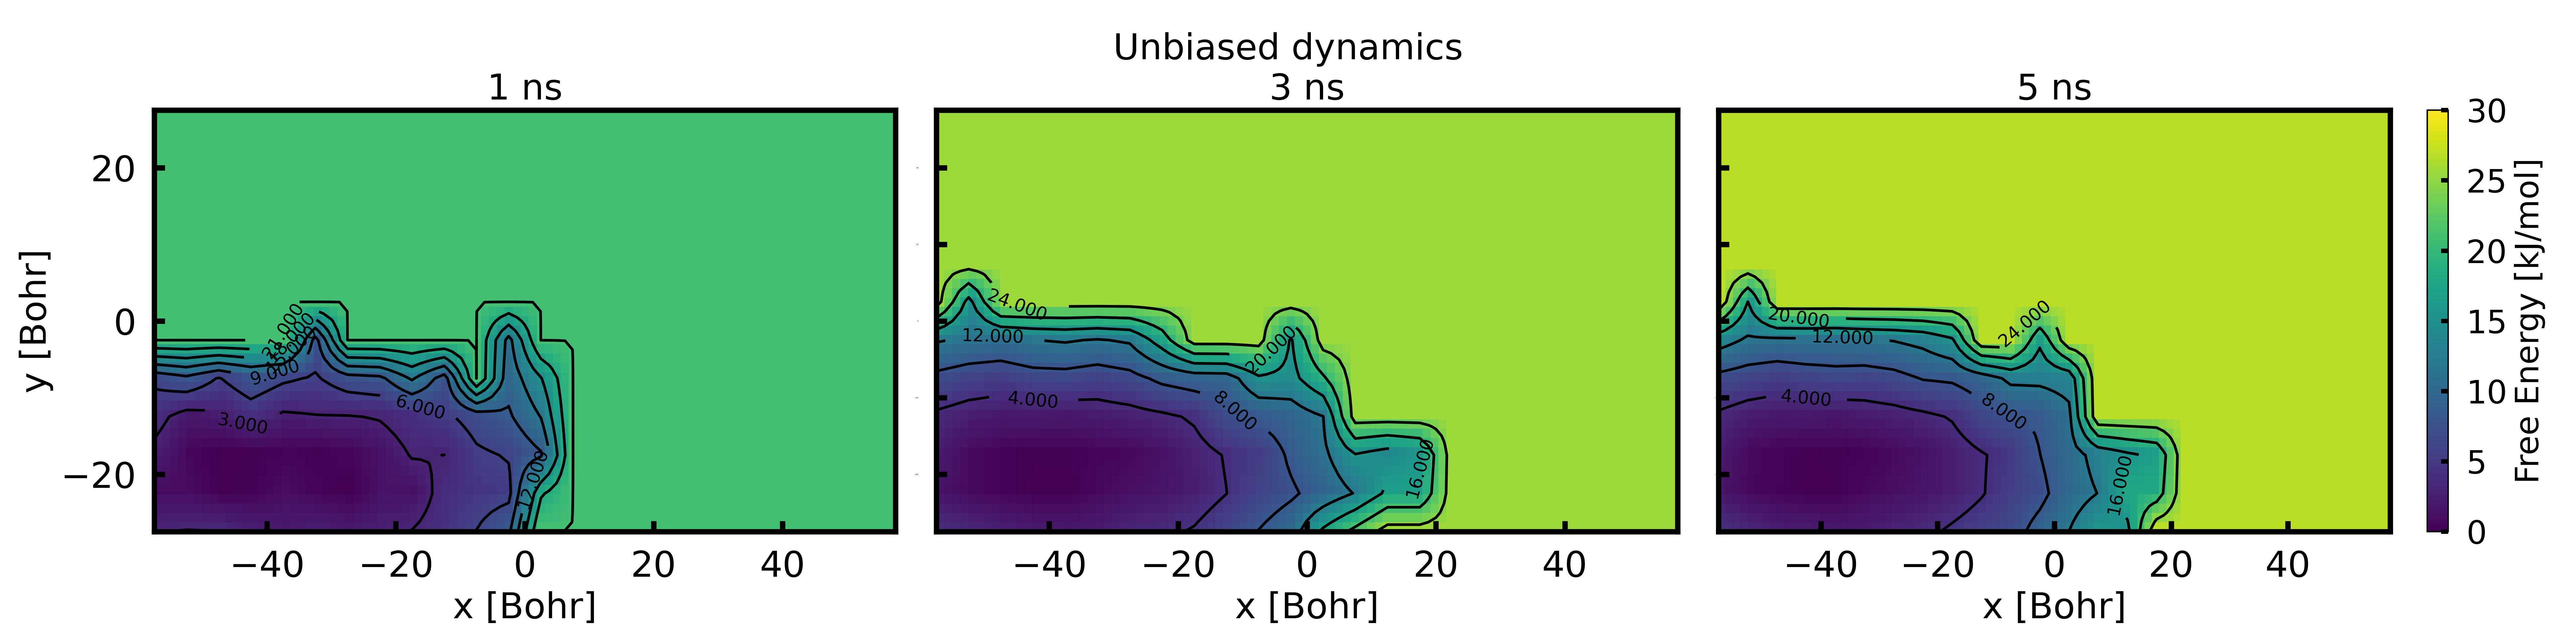
\includegraphics[width=0.95\textwidth]{bilder/test_2D/reference_freeE} \\
  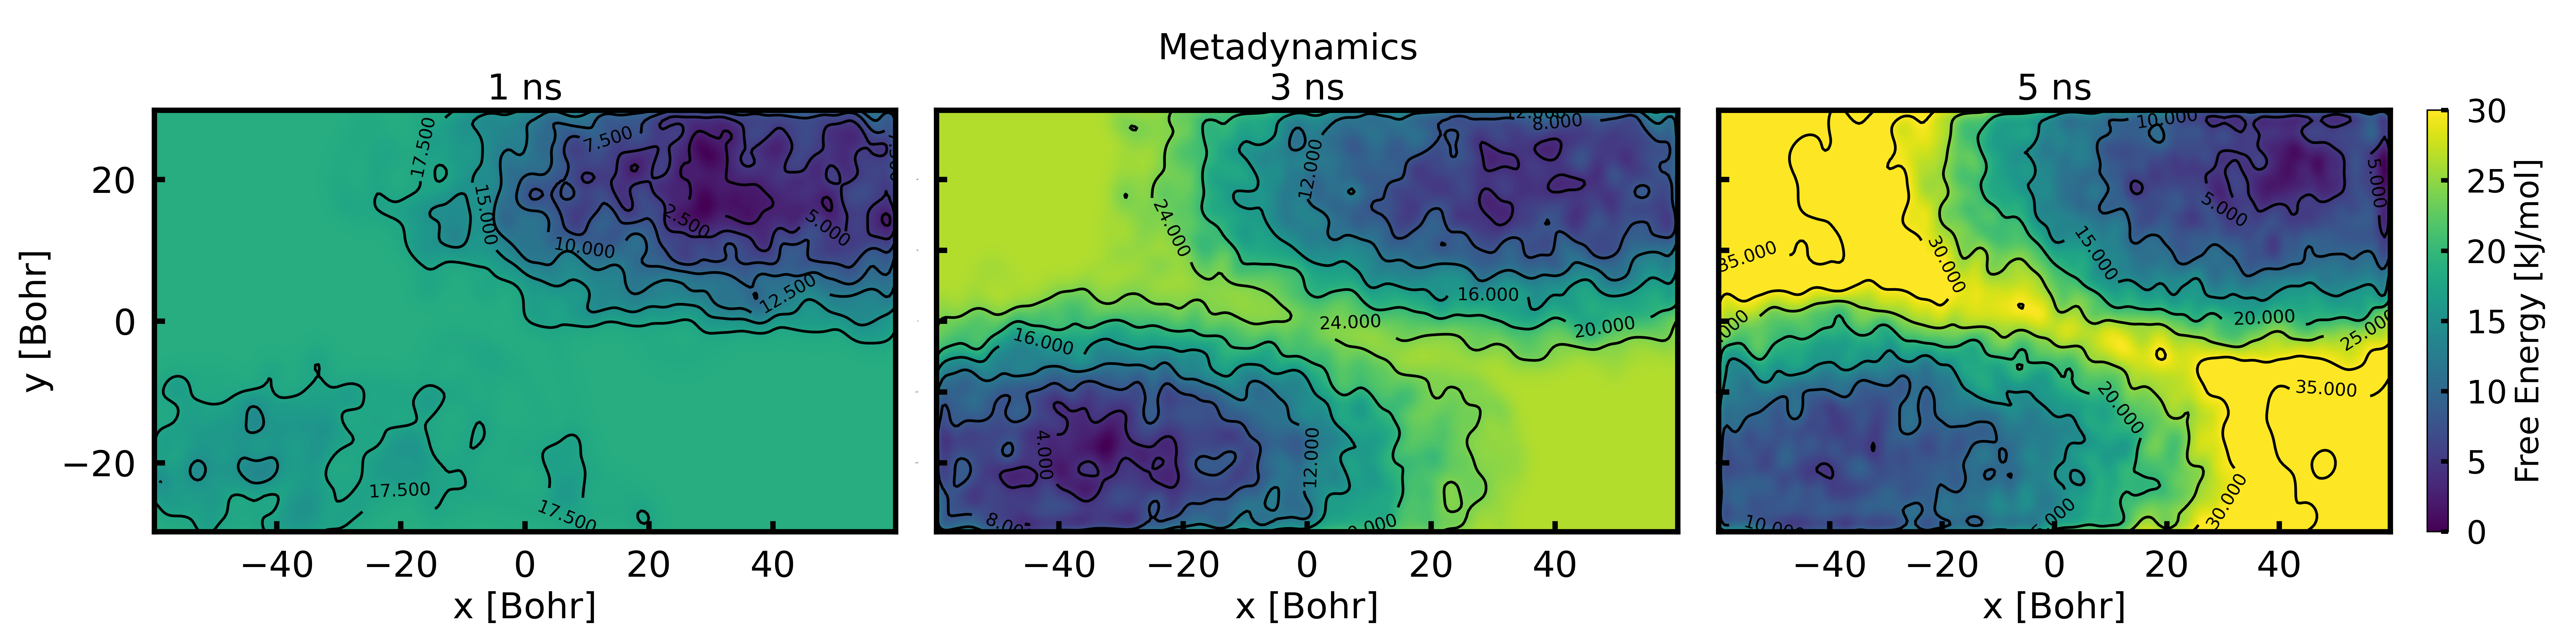
\includegraphics[width=0.95\textwidth]{bilder/test_2D/metaD_freeE} \\
  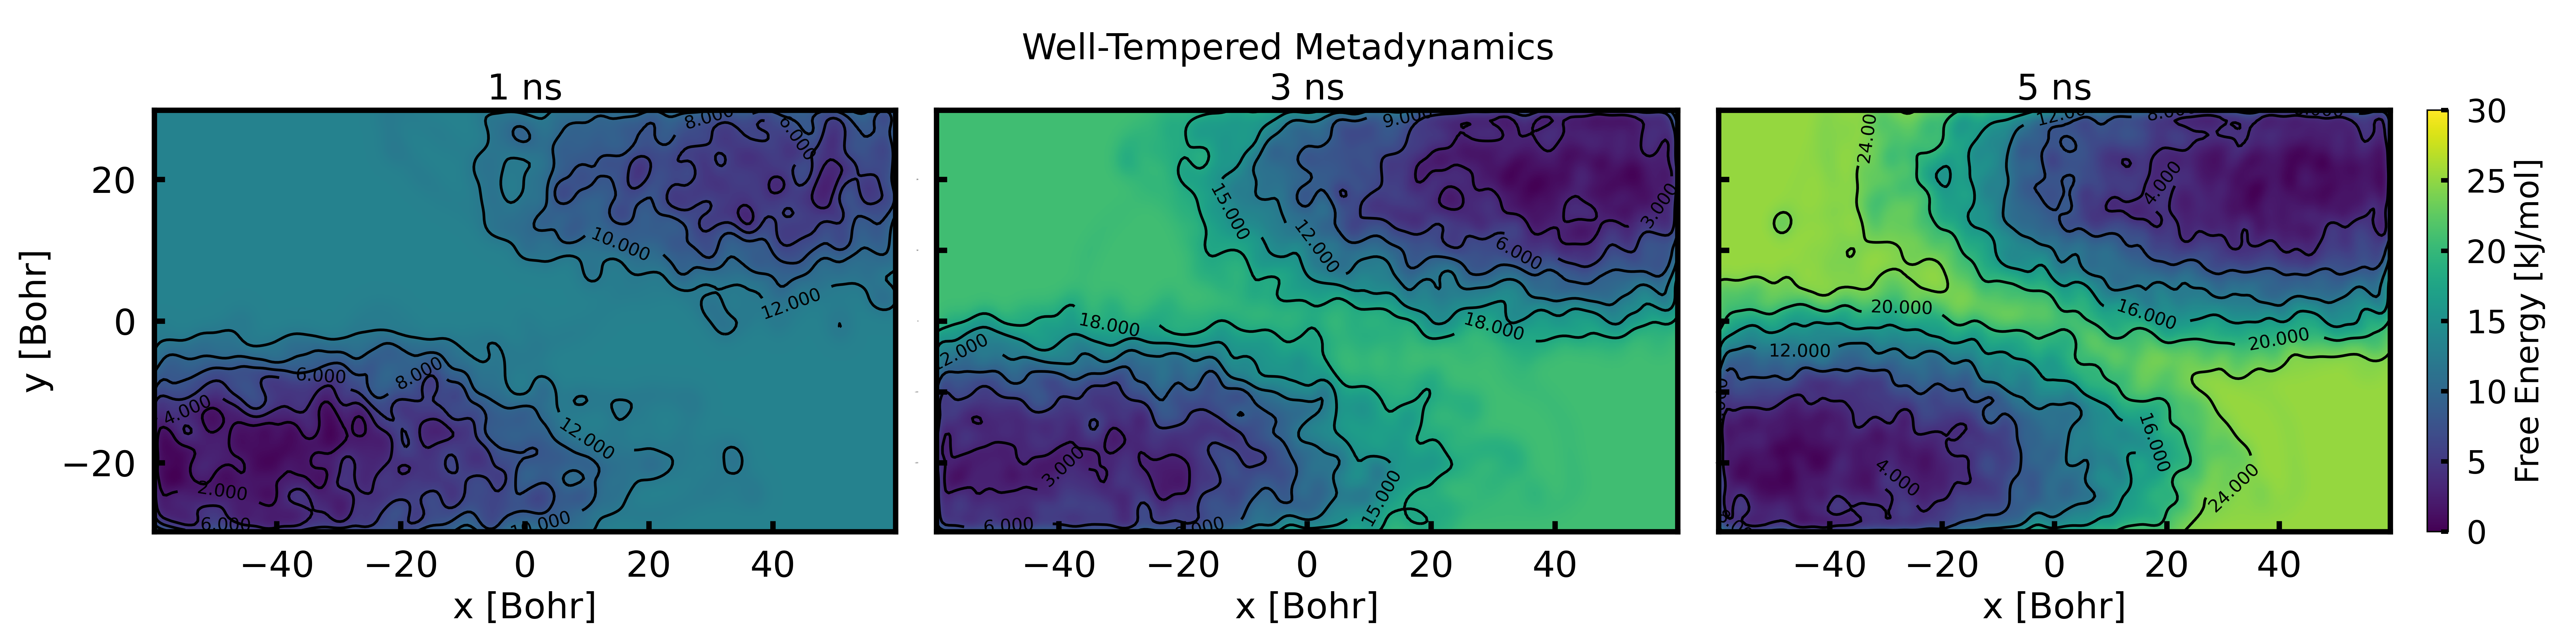
\includegraphics[width=0.95\textwidth]{bilder/test_2D/WTM_freeE} \\
  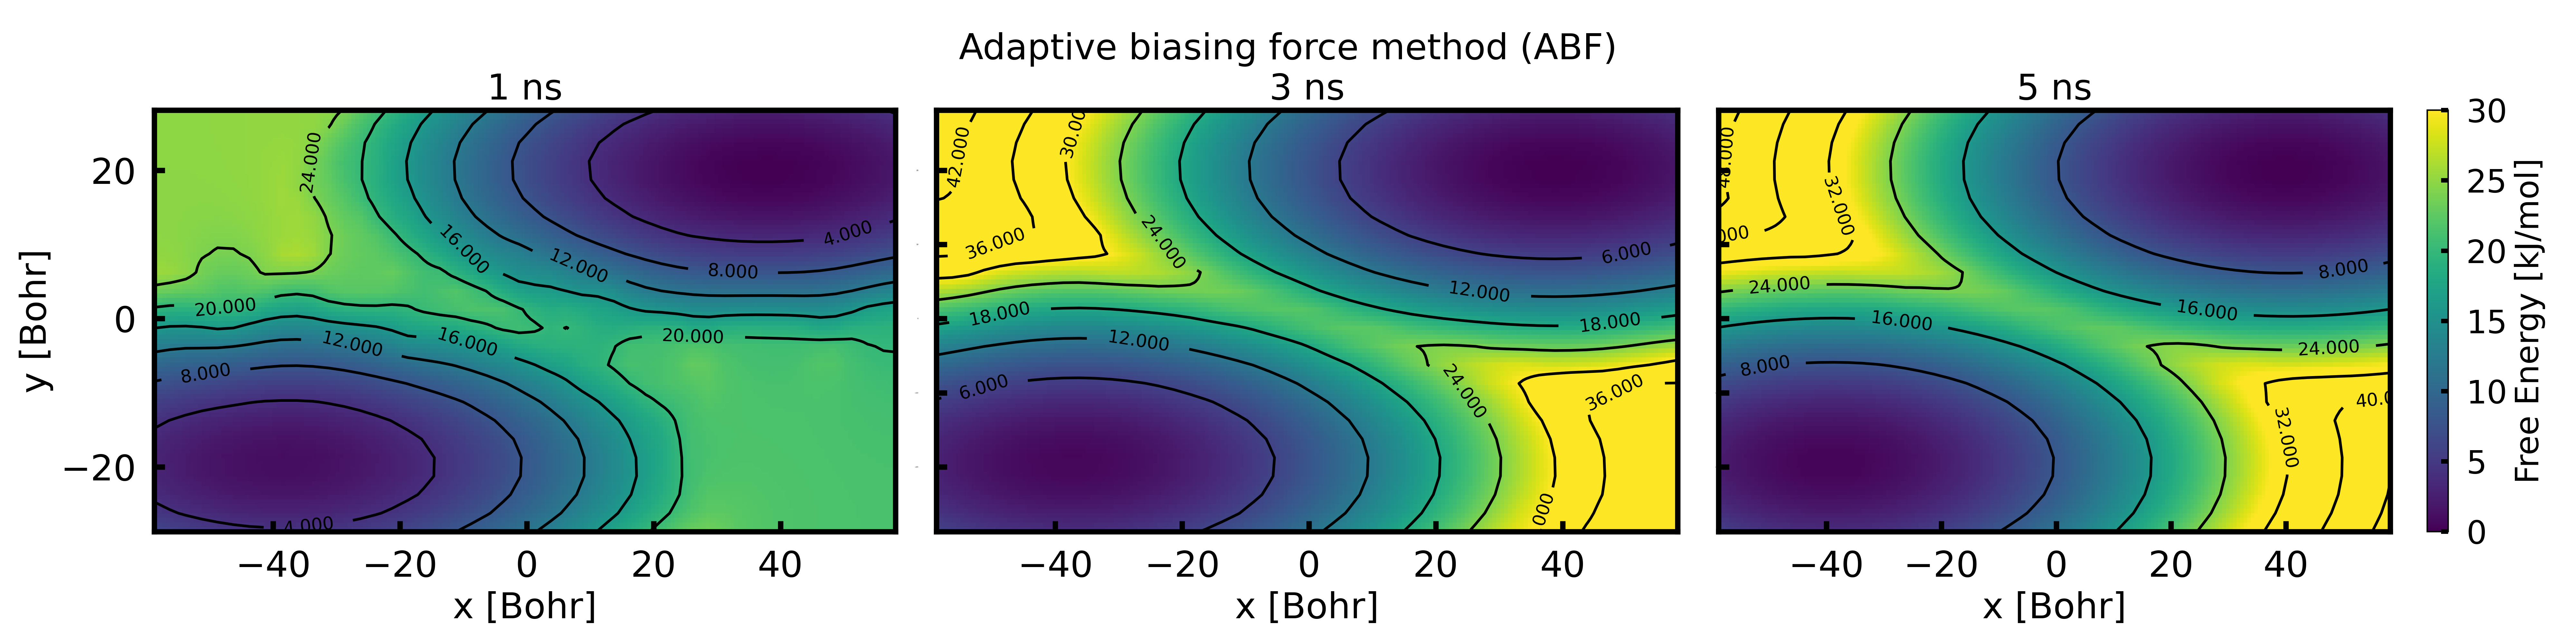
\includegraphics[width=0.95\textwidth]{bilder/test_2D/ABF_freeE}  \\
  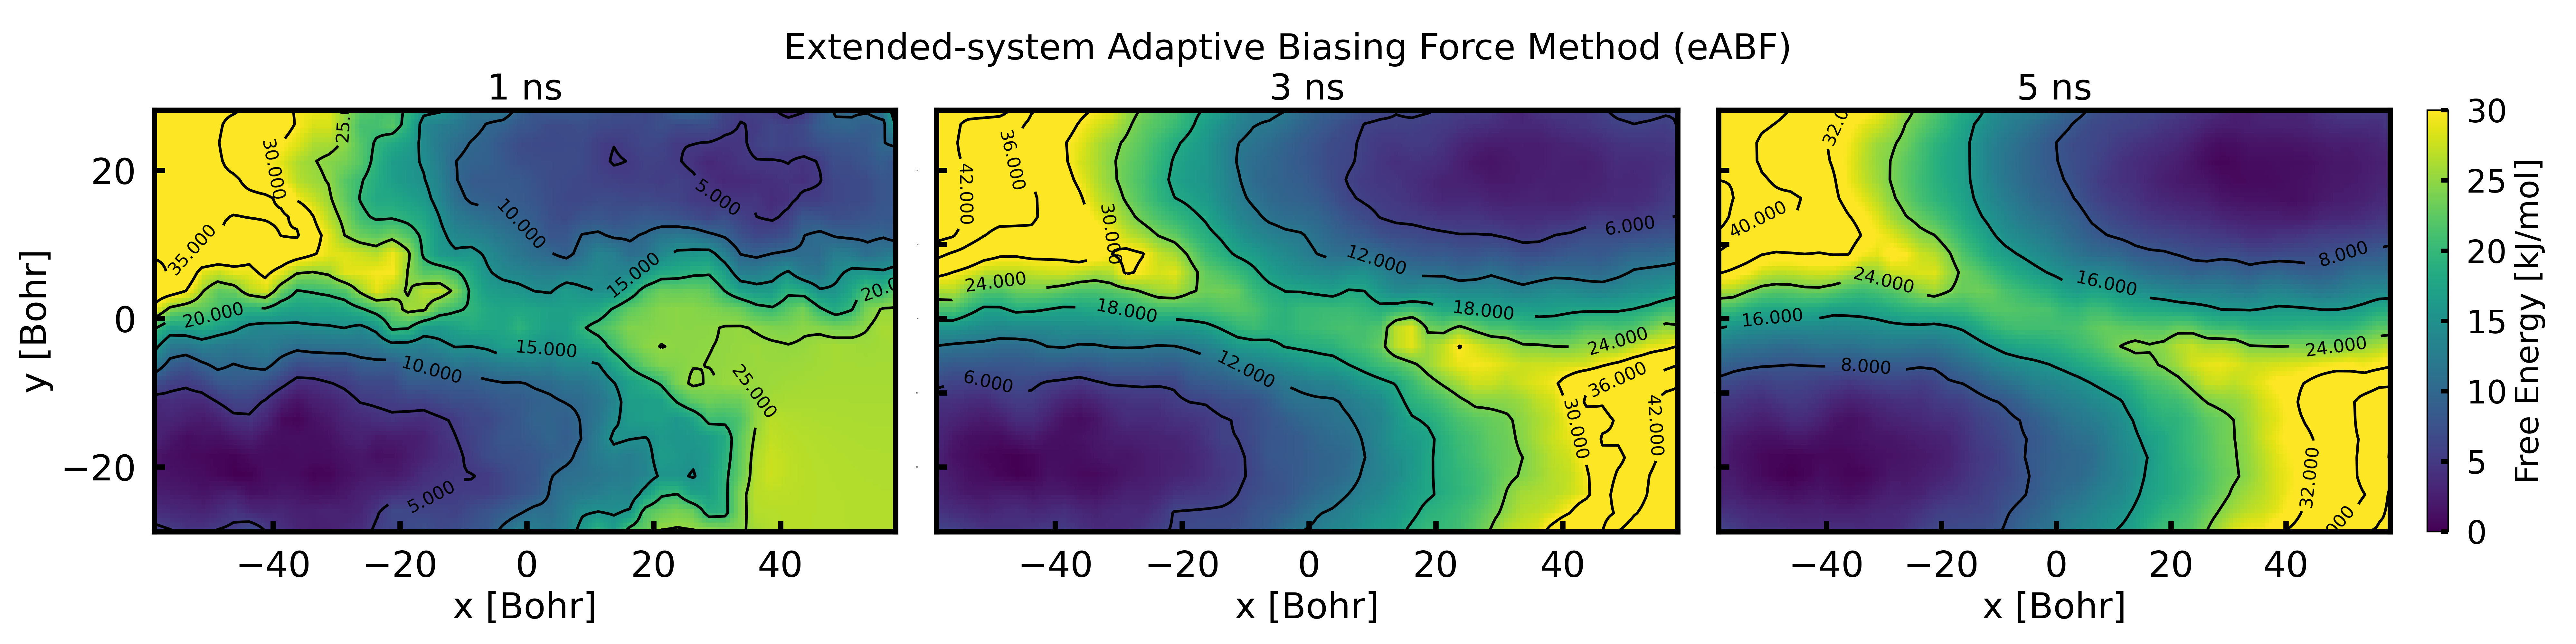
\includegraphics[width=0.95\textwidth]{bilder/test_2D/eABF_freeE} \\
  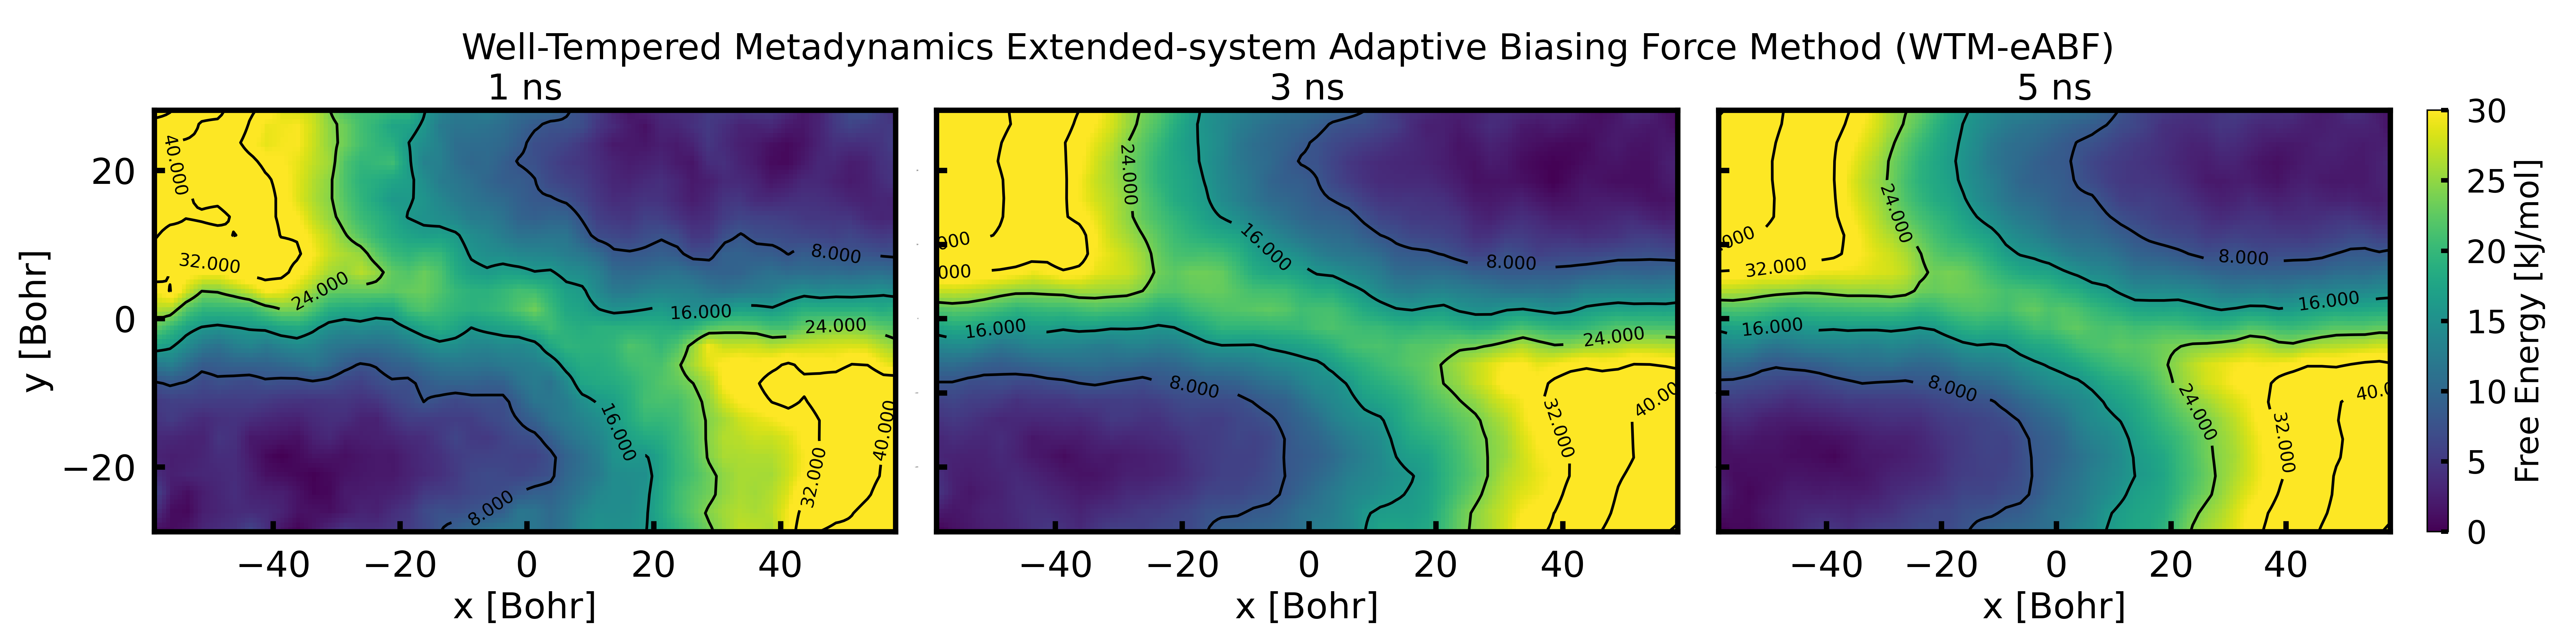
\includegraphics[width=0.95\textwidth]{bilder/test_2D/meta_eABF_freeE}
  \caption{
  Snapshot of the PMFs computed from a single trajectory with unbiased dynamics and different adaptive biasing algorithms after 1, 3 and 5~ns in potential $U_2$. Details are given in the appendix.}
\label{fig:2D ABF}%
\end{figure}
